\documentclass[12pt,a4paper, spanish]{article}
\usepackage[spanish]{babel}
\usepackage[utf8]{inputenc}
\usepackage{setspace}
\usepackage[
  pdftex,
  pdfauthor={--- Arturo Vidal Peña & Javier Melero Deza ---},
  pdftitle={--- Práctica RESTful 2018/2019 ---},
  hidelinks]{hyperref}

% --- IMAGES ---
\usepackage[pdftex]{graphicx}
\usepackage{subfigure}
\usepackage{graphicx}
\usepackage{float}
\usepackage[usenames,dvipsnames]{color}
\DeclareGraphicsExtensions{.png,.jpg,.pdf,.mps,.gif,.bmp}
% --- IMAGES ---

% --- TABLES ---
\usepackage{multirow}
% --- TABLES ---

% --- CODE ---
\usepackage{listings}
\definecolor{backcolour}{RGB}{45,45,45}
\definecolor{keycolour}{RGB}{242, 119, 122}
\definecolor{valuecolour}{RGB}{204,204,204}
\definecolor{stringcolour}{RGB}{153,204,153}
\definecolor{integercolour}{RGB}{249,145,87}

\definecolor{codegray}{rgb}{0.5,0.5,0.5}

\newcommand\YAMLcolonstyle{\color{keycolour}\mdseries}
\newcommand\YAMLkeystyle{\color{keycolour}\bfseries}
\newcommand\YAMLvaluestyle{\color{valuecolour}\mdseries}
\newcommand\YAMLstringstyle{\color{stringcolour}\mdseries}
\newcommand\YAMLintegerstyle{\color{integercolour}\mdseries}

\makeatletter

% here is a macro expanding to the name of the language
% (handy if you decide to change it further down the road)
\newcommand\language@yaml{yaml}

\expandafter\expandafter\expandafter\lstdefinelanguage
\expandafter{\language@yaml}
{
	numbers=left,                    
	numbersep=5pt, 
	numberstyle=\tiny\color{codegray},
	backgroundcolor=\color{backcolour},
	breaklines=true,
	keywords={true, false, null,y,n},
	keywordstyle=\color{integercolour}\bfseries,
	basicstyle=\YAMLkeystyle,                     % assuming a key comes first
	sensitive=false,
	captionpos=b,
	comment=[l]{\#},
	morecomment=[s]{/*}{*/},
	commentstyle=\color{purple}\ttfamily,
	stringstyle=\YAMLstringstyle\ttfamily,
	moredelim=[l][\color{orange}]{\&},
	moredelim=[l][\color{magenta}]{*},
	moredelim=**[il][\YAMLcolonstyle{:}\YAMLvaluestyle]{:},   % switch to value style at :
	morestring=[b]',
	morestring=[b]",
	literate =    {---}{{\ProcessThreeDashes}}3
	{>}{{\textcolor{red}\textgreater}}1     
	{|}{{\textcolor{red}\textbar}}1 
	{\ -\ }{{\mdseries\ -\ }}3,
	showstringspaces=false,
}

% switch to key style at EOL
\lst@AddToHook{EveryLine}{\ifx\lst@language\language@yaml\YAMLkeystyle\fi}
\makeatother

\newcommand\ProcessThreeDashes{\llap{\color{cyan}\mdseries-{-}-}}
% --- CODE ---

% --- MARGIN DIMENSIONS ---
\frenchspacing \addtolength{\hoffset}{-1.5cm}
\addtolength{\textwidth}{3cm} \addtolength{\voffset}{-2.5cm}
\addtolength{\textheight}{4cm}
\setlength{\headheight}{15pt}
% --- MARGIN DIMENSIONS ---

% --- TITLE DATA ---
\title{\textbf{Práctica RESTful} \\
       \textsc{Sistemas Orientados a Servicios} \\
       \emph{DLSIIS}}
\author{\emph{Vidal Peña, Arturo}\\
        \emph{Melero Deza, Javier}}
\date{\underline{\today}}
% --- TITLE DATA ---

% --- TABLE OF CONTENTS' DOTS
\usepackage{tocloft}
\renewcommand{\cftsecleader}{\cftdotfill{\cftdotsep}}
% --- TABLE OF CONTENTS' DOTS

% --- DOCUMENT ---
\begin{document}

% --- TITLE ---
\maketitle
\thispagestyle{empty}
\pagenumbering{gobble}
\renewcommand*\contentsname{Índice de contenidos}
\tableofcontents
\pagebreak
% --- TITLE ---

\pagenumbering{arabic}

\section{Resumen del diseño del servicio}
	\begin{figure}[H]
		\centering
		\includegraphics[width=\textwidth]{images/yaml/index.png}
	\end{figure}
\subsection{Métodos de usuarios}
\subsubsection{Crear un usuario}
\begin{figure}[H]
	\centering
	\includegraphics[width=\textwidth]{images/yaml/userOps/post.png}
\end{figure}
\subsubsection{Obtener info del usuario}
\begin{figure}[H]
	\centering
	\includegraphics[width=\textwidth]{images/yaml/userOps/getUser.png}
\end{figure}
\subsubsection{Obtener todos los usuarios}
\begin{figure}[H]
	\centering
	\includegraphics[width=\textwidth]{images/yaml/userOps/get.png}
\end{figure}
\subsubsection{Modificar un usuario}
\begin{figure}[H]
	\centering
	\includegraphics[width=\textwidth]{images/yaml/userOps/put.png}
\end{figure}
\subsubsection{Eliminar un usuario}
\begin{figure}[H]
	\centering
	\includegraphics[width=\textwidth]{images/yaml/userOps/delete.png}
\end{figure}

\newpage
\subsection{Métodos de amistad}
\subsubsection{Crear una amistad}
\begin{figure}[H]
	\centering
	\includegraphics[width=\textwidth]{images/yaml/userFriendOps/post.png}
\end{figure}
\subsubsection{Obtener amigos de un usuario}
\begin{figure}[H]
	\centering
	\includegraphics[width=\textwidth]{images/yaml/userFriendOps/get.png}
\end{figure}

\newpage
\subsection{Métodos de mensajes}
\subsubsection{Crear un mensaje}
\begin{figure}[H]
	\centering
	\includegraphics[width=\textwidth]{images/yaml/msgOps/post.png}
\end{figure}
\subsubsection{Obtener info del mensaje}
\begin{figure}[H]
	\centering
	\includegraphics[width=\textwidth]{images/yaml/msgOps/getMsg.png}
\end{figure}
\subsubsection{Obtener todos los mensajes de un usuario}
\begin{figure}[H]
	\centering
	\includegraphics[width=\textwidth]{images/yaml/msgOps/get.png}
\end{figure}
\subsubsection{Modificar un mensaje}
\begin{figure}[H]
	\centering
	\includegraphics[width=\textwidth]{images/yaml/msgOps/put.png}
\end{figure}
\subsubsection{Eliminar un mensaje}
\begin{figure}[H]
	\centering
	\includegraphics[width=\textwidth]{images/yaml/msgOps/delete.png}
\end{figure}

\newpage
\subsection{Métodos de mensajes privados}
\subsubsection{Crear un mensaje privado}
\begin{figure}[H]
	\centering
	\includegraphics[width=\textwidth]{images/yaml/privateMsgOps/post.png}
\end{figure}
\subsubsection{Obtener info del mensaje privado}
\begin{figure}[H]
	\centering
	\includegraphics[width=\textwidth]{images/yaml/privateMsgOps/getMsg.png}
\end{figure}
\subsubsection{Obtener todos los mensajes privados de un usuario}
\begin{figure}[H]
	\centering
	\includegraphics[width=\textwidth]{images/yaml/privateMsgOps/get.png}
\end{figure}

\newpage
\subsection{Fichero YAML del servicio}
El siguiente código se ha realizado usando la herramienta Swagger Editor. El fichero se encuentra adjunto a este documento y las capturas previas. 
\lstinputlisting[language=YAML]{yaml/config.yaml}

\newpage
\subsubsection{Definición de los métodos de usuario}
\lstinputlisting[language=YAML]{yaml/usuarios.yaml}

\newpage
\subsubsection{Definición de los métodos de mensajes}
\lstinputlisting[language=YAML]{yaml/mensajes.yaml}

\newpage
\subsubsection{Definición de los métodos de mensajes privados}
\lstinputlisting[language=YAML]{yaml/privados.yaml}

\newpage
\subsubsection{Definición de los métodos de amistades}
\lstinputlisting[language=YAML]{yaml/amigos.yaml}

\newpage
\subsubsection{Definición de los esquemas}
\lstinputlisting[language=YAML]{yaml/components.yaml}

\newpage
\section{Capturas de la ejecución en el cliente Postman}
Hay que poner detalles tanto de la invocación como del resultado de la operación.

\subsection{Métodos de usuarios}
\subsubsection{POST}
\begin{figure}[H]
	\centering
	\includegraphics[width=0.75\textwidth]{images/Usuarios/POST/postRaquel.png}
	\caption{Se añade el usuario 1 de nombre Raquel.}
\end{figure}

\begin{figure}[H]
	\centering
	\includegraphics[width=0.75\textwidth]{images/Usuarios/POST/postJavi.png}
	\caption{Se añade el usuario 2 de nombre Javi.}
\end{figure}

\begin{figure}[H]
	\centering
	\includegraphics[width=0.75\textwidth]{images/Usuarios/POST/postRafa.png}
	\caption{Se añade el usuario 3 de nombre Rafa.}
\end{figure}

\begin{figure}[H]
	\centering
	\includegraphics[width=0.75\textwidth]{images/Usuarios/POST/postMaria.png}
	\caption{Se añade el usuario 4 de nombre María.}
\end{figure}
\newpage
\subsubsection{GET}

\begin{figure}[H]
	\centering
	\includegraphics[width=0.75\textwidth]{images/Usuarios/GET/getUsuarios.png}
	\caption{Se obtienen todos los usuarios.}
\end{figure}

\begin{figure}[H]
	\centering
	\includegraphics[width=0.75\textwidth]{images/Usuarios/GET/getAfterPut.png}
	\caption{Obtención del usuario 3 después de ser modificado.}
\end{figure}

\begin{figure}[H]
	\centering
	\includegraphics[width=0.75\textwidth]{images/Usuarios/GET/getAfterDelete.png}
	\caption{Se obtienen todos los usuarios después de eliminar el usuario 4 (Figura 10).}
\end{figure}

\subsubsection{PUT}
\begin{figure}[H]
	\centering
	\includegraphics[width=0.75\textwidth]{images/Usuarios/PUT/putRafa.png}
	\caption{Modificación del nombre de usuario 3.}
\end{figure}

\begin{figure}[H]
	\centering
	\includegraphics[width=0.75\textwidth]{images/Usuarios/PUT/getAfterPutRafa.png}
	\caption{Obtención de los datos después de la modificación anterior.}
\end{figure}

\subsubsection{DELETE}
\begin{figure}[H]
	\centering
	\includegraphics[width=0.75\textwidth]{images/Usuarios/DELETE/deleteMaria.png}
	\caption{Eliminación del usuario 4.}
\end{figure}
\newpage

\subsection{Métodos de mensajes}
\subsubsection{POST}
\begin{figure}[H]
	\centering
	\includegraphics[width=0.75\textwidth]{images/Mensajes/POST/postMensaje1.png}
	\caption{Creación del mensaje 1 asociado al usuario 1.}
\end{figure}

\begin{figure}[H]
	\centering
	\includegraphics[width=0.75\textwidth]{images/Mensajes/POST/postMensaje2.png}
	\caption{Creación del mensaje 2 asociado al usuario 2.}
\end{figure}

\begin{figure}[H]
	\centering
	\includegraphics[width=0.75\textwidth]{images/Mensajes/POST/postMensaje4.png}
	\caption{Creación del mensaje 4 asociado al usuario 1.}
\end{figure}
\newpage
\subsubsection{GET}

\begin{figure}[H]
	\centering
	\includegraphics[width=0.75\textwidth]{images/Mensajes/GET/getMensajes1.png}
	\caption{Se obtienen todos mensajes asociados al usuario 1.}
\end{figure}

\begin{figure}[H]
	\centering
	\includegraphics[width=0.75\textwidth]{images/Mensajes/GET/getMensaje.png}
	\caption{Obtención del mensaje 1 del usuario 1.}
\end{figure}

\begin{figure}[H]
	\centering
	\includegraphics[width=0.75\textwidth]{images/Mensajes/GET/getAfterPut.png}
	\caption{Obtención del mensaje 4 después de ser modificado (Figura 17).}
\end{figure}

\subsubsection{PUT}
\begin{figure}[H]
	\centering
	\includegraphics[width=0.75\textwidth]{images/Mensajes/PUT/putMensaje.png}
	\caption{Modificación del mensaje 4 asociado al usuario 1.}
\end{figure}

\subsubsection{DELETE}
\begin{figure}[H]
	\centering
	\includegraphics[width=0.75\textwidth]{images/Mensajes/DELETE/deleteMensaje.png}
	\caption{Eliminación del mensaje 1 del usuario 1.}
\end{figure}
\newpage

\subsection{Métodos de Mensajes Privados}
\subsubsection{POST}
\begin{figure}[H]
	\centering
	\includegraphics[width=0.75\textwidth]{images/Privados/POST/postCuartoPrivado.png}
	\caption{Creación del cuarto mensaje privado del usuario 1 al 3.}
\end{figure}

\subsubsection{GET}
\begin{figure}[H]
	\centering
	\includegraphics[width=0.75\textwidth]{images/Privados/GET/getPrivados.png}
	\caption{Obtención de todos los mensajes privados escritos por el usuario 3.}
\end{figure}

\begin{figure}[H]
	\centering
	\includegraphics[width=0.75\textwidth]{images/Privados/GET/getPrivado3.png}
	\caption{Obtención del mensaje privado 4 del usuario 3.}
\end{figure}

\newpage
\subsection{Métodos de Amistad}
\subsubsection{POST}
\begin{figure}[H]
	\centering
	\includegraphics[width=0.75\textwidth]{images/Amistad/POST/postAmigo.png}
	\caption{Se añade el usuario 3 como amigo del usuario 1.}
\end{figure}

\begin{figure}[H]
	\centering
	\includegraphics[width=0.75\textwidth]{images/Amistad/POST/postAmigo2.png}
	\caption{Se añade el usuario 1 como amigo del usuario 2.}
\end{figure}

\newpage
\subsubsection{GET}

\begin{figure}[H]
	\centering
	\includegraphics[width=0.75\textwidth]{images/Amistad/GET/getAmigos1.png}
	\caption{Obtención de todos los usuarios amigos del usuario 1.}
\end{figure}

\begin{figure}[H]
	\centering
	\includegraphics[width=0.75\textwidth]{images/Amistad/GET/getAmigo3.png}
	\caption{Obtención de todos los usuarios amigos del usuario 3.}
\end{figure}

\begin{figure}[H]
	\centering
	\includegraphics[width=0.75\textwidth]{images/Amistad/GET/getAfterDelete.png}
	\caption{Obtención de los amigos del usuario 1 después de eliminar uno de ellos (Figura 27).}
\end{figure}

\subsubsection{DELETE}
\begin{figure}[H]
	\centering
	\includegraphics[width=0.75\textwidth]{images/Amistad/DELETE/removeFriend.png}
	\caption{Eliminación del usuario 2 de los amigos del usuario 1.}
\end{figure}
\newpage

\subsection{Obtención de mensajes similar a FaceBook}
\begin{figure}[H]
	\centering
	\includegraphics[width=0.75\textwidth]{images/MensajesFacebook/amistadPostParaVerPosts.png}
	\caption{Obtención de los amigos del usuario 1.}
\end{figure}

\begin{figure}[H]
	\centering
	\includegraphics[width=0.75\textwidth]{images/MensajesFacebook/postMensajePrueba.png}
	\caption{Creación de un mensaje del usuario 2.}
\end{figure}

\begin{figure}[H]
	\centering
	\includegraphics[width=0.75\textwidth]{images/MensajesFacebook/getMensajesAmigos.png}
	\caption{Obtención de los mensajes de los amigos del usuario 1.}
\end{figure}

\subsection{Aplicación móvil}
\begin{figure}[H]
	\centering
	\includegraphics[width=0.75\textwidth]{images/AplicacionMovil/movilDisplay.png}
	\caption{Obtención de la información del usuario 1 simulando una aplicación móvil.}
\end{figure}
\newpage
\section{ANEXO: Problemas encontrados}

Los fallos encontrados referentes a la Máquina virtual son:

\begin{itemize}
	\item Con la aplicación Postman, al probar los métodos HTTP.
	\item Con la aplicación Eclipse, que algunas veces no encontraba las URIs implementadas.
	\item Con la baja calidad de las capturas de pantalla del SO utilizado (probablemente por la antigüedad del mismo).
\end{itemize} 

\begin{figure}[H]
	\centering
	\subfigure{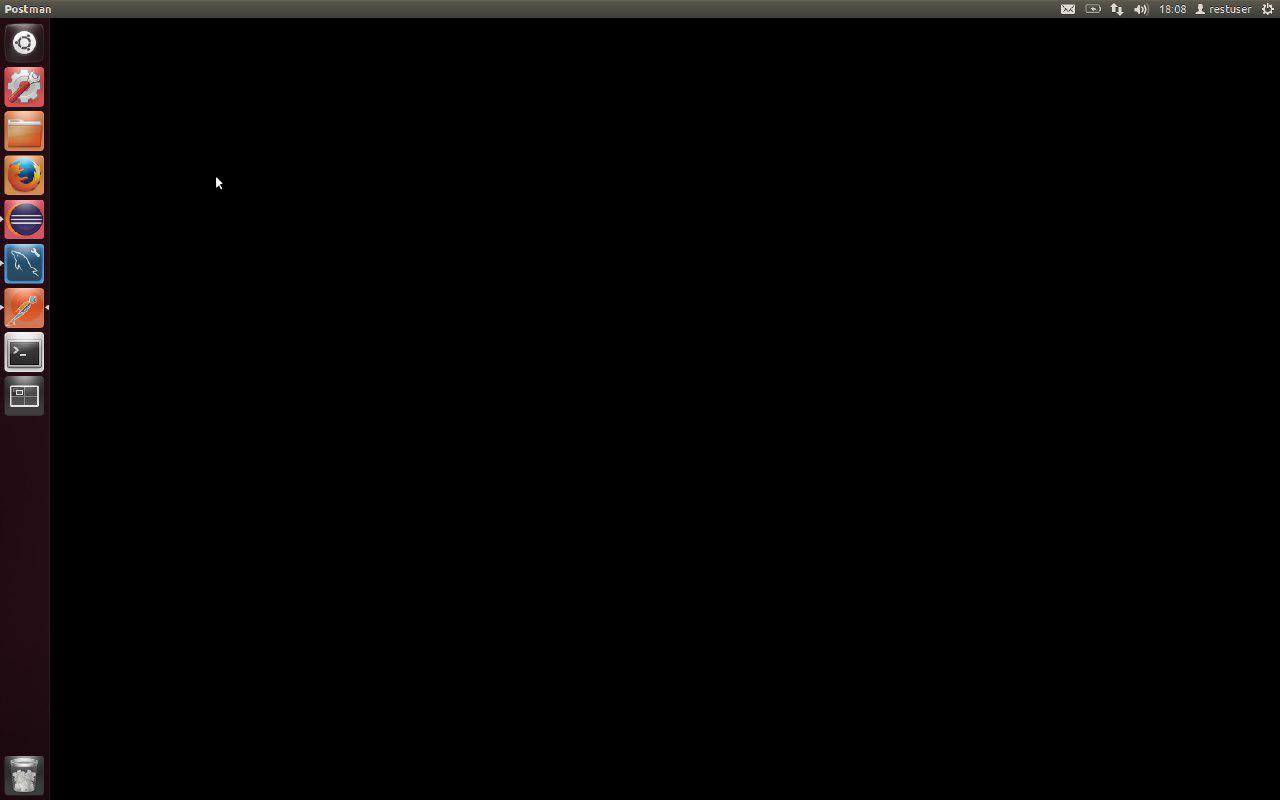
\includegraphics[width=0.45\textwidth]{images_old/error1.jpg}}
	\subfigure{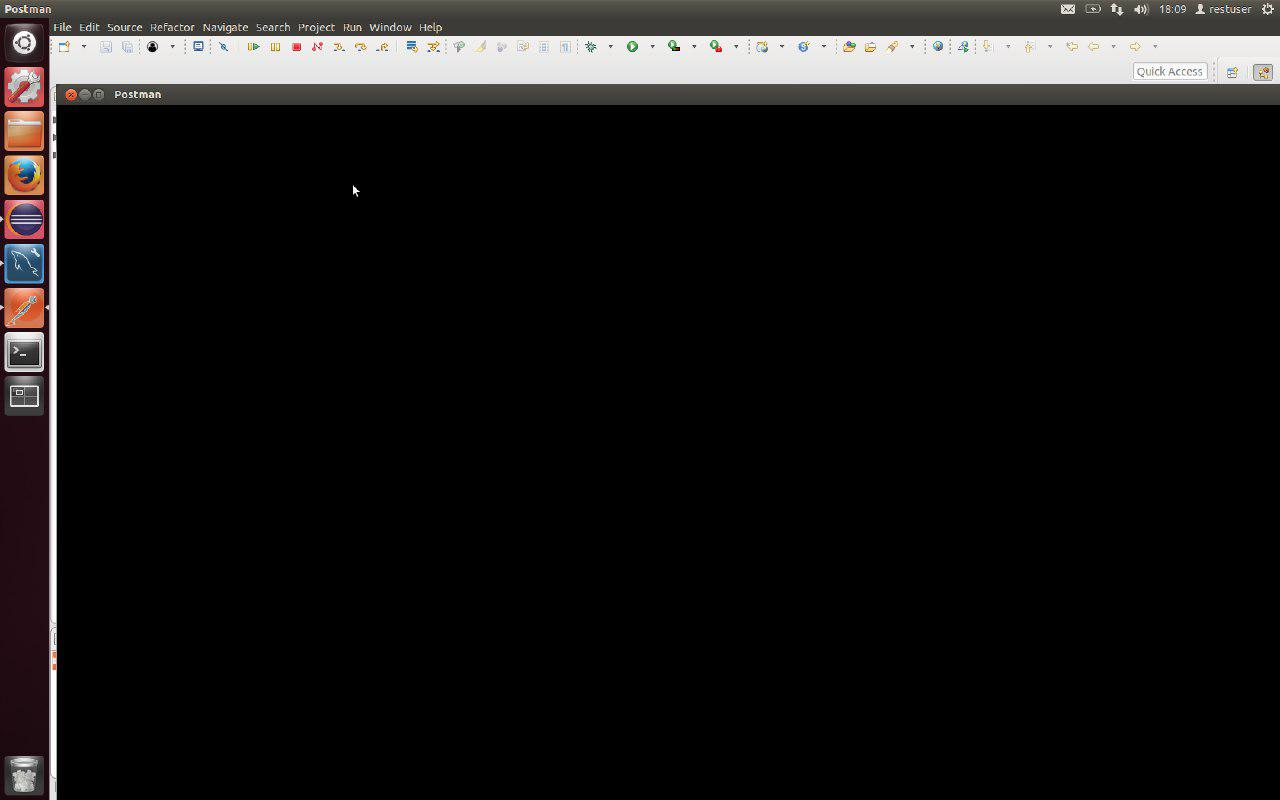
\includegraphics[width=0.45\textwidth]{images_old/error2.jpg}}
	\caption{Fallo de la aplicación Postman al probar métodos.}
\end{figure}



\end{document}
% --- DOCUMENT ---
